\subsection{اسلاید های دیجیتال}\label{subsec:اسلاید-های-دیجیتال}
همانطور که در قسمت قبل گفته شد، نمونه های تهیه شده از ناحیه های مشکوک بیمار از غده تیروئید، توسط دستگاه هایی اسکن می شوند و به صورت تصاویری دیجیتال در می آیند که برای کامپیوتر های قابل خواندن هستند.
قبل از اینکه این نمونه ها توسط دستگاه اسکن شوند ممکن است فرآیندی روی نمونه ها انجام شود تا سلول ها در زیر میکروسکپ و یا در تصویر دیجیتال به خود رنگ بگیرند.
این کار به متخصصین کمک می کنند تا سلول ها را راحت تر از دیگر مواد داخل نمونه تشخیص دهند و این باعث افزایش دقت تشخیص می شود.
به همین دلیل اسلاید های تهیه شده به این روش، ممکن است رنگ های مختلفی به خود بگیرند.


نمونه ای از این اسلاید ها در شکل ~\autoref{fig:sampleWSIscan} آمده است.
\begin{figure}
    \begin{center}
        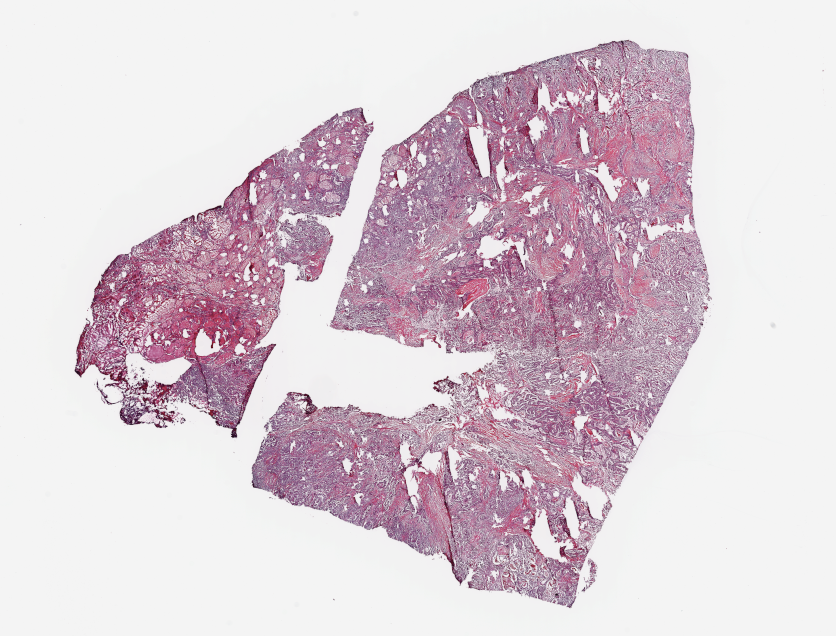
\includegraphics[width=\linewidth]{figs/introduction/Sample_WSI.PNG}
    \end{center}
    \caption{نمونه اسلاید اسکن شده از غده تیروئید}
    \label{fig:sampleWSIscan}
\end{figure}
این اسلاید ها معمولا ابعاد بسیار بزرگی دارند و ممکن است تا بزرگنمایی 40 برابر را پشتیبانی کنند.
به همین دلیل ممکن است حجمی بین چند مگابایت تا چند گیگابایت را به خود بگیرند.

مدل هوش مصنوعی که در این پژوهش توسعه داده می شود، باید قادر باشد ویژگی های سلول ها را از روی این اسلاید ها تشخیص داده و تخمین درستی از وضعیت سرطان به ما بدهد.